\chapter{Beispielkapitel}
\label{cha:beispielkapitel}
Dieses Beispielkapitel dient der Darstellung häufig verwendeter Elemente in LaTeX wie Aufzählungen, Abbildungen, Tabellen oder Gleichungen. Es hat keinen Anspruch auf Vollständigkeit und kann gerne erweitert werden. Eine ausführliche Beschreibung der LaTeX-Befehle kann der Befehlsübersicht entnommen werden.
Die  Beispiele können kopiert und dann angepasst werden.  
% Abschnitt 1 --------------------------------------------------------------
% 		Name des Abschnittes
% --------------------------------------------------------------------------
\section{Aufzählungen}
\label{sec:aufzaehlungen}

\subsection{Aufzählungen mit Punkten}
\label{aufzaehlung_punkte}

\begin{itemize}
	\item Körper
	\item Bindungselemente
	\item Koppelelemente
\end{itemize}

\subsection{Aufzählungen mit Zahlen}
\label{aufzaehlung_zaheln}

\begin{enumerate}
	\item Körper
	\item Bindungselemente
	\item Koppelelemente
\end{enumerate}

\cleardoublepage
% Abschnitt 2 --------------------------------------------------------------
% 		Name des Abschnittes
% --------------------------------------------------------------------------
\section{Abbildungen}
\label{sec:abbildungen}

\begin{figure}[htbp]
	\centering
		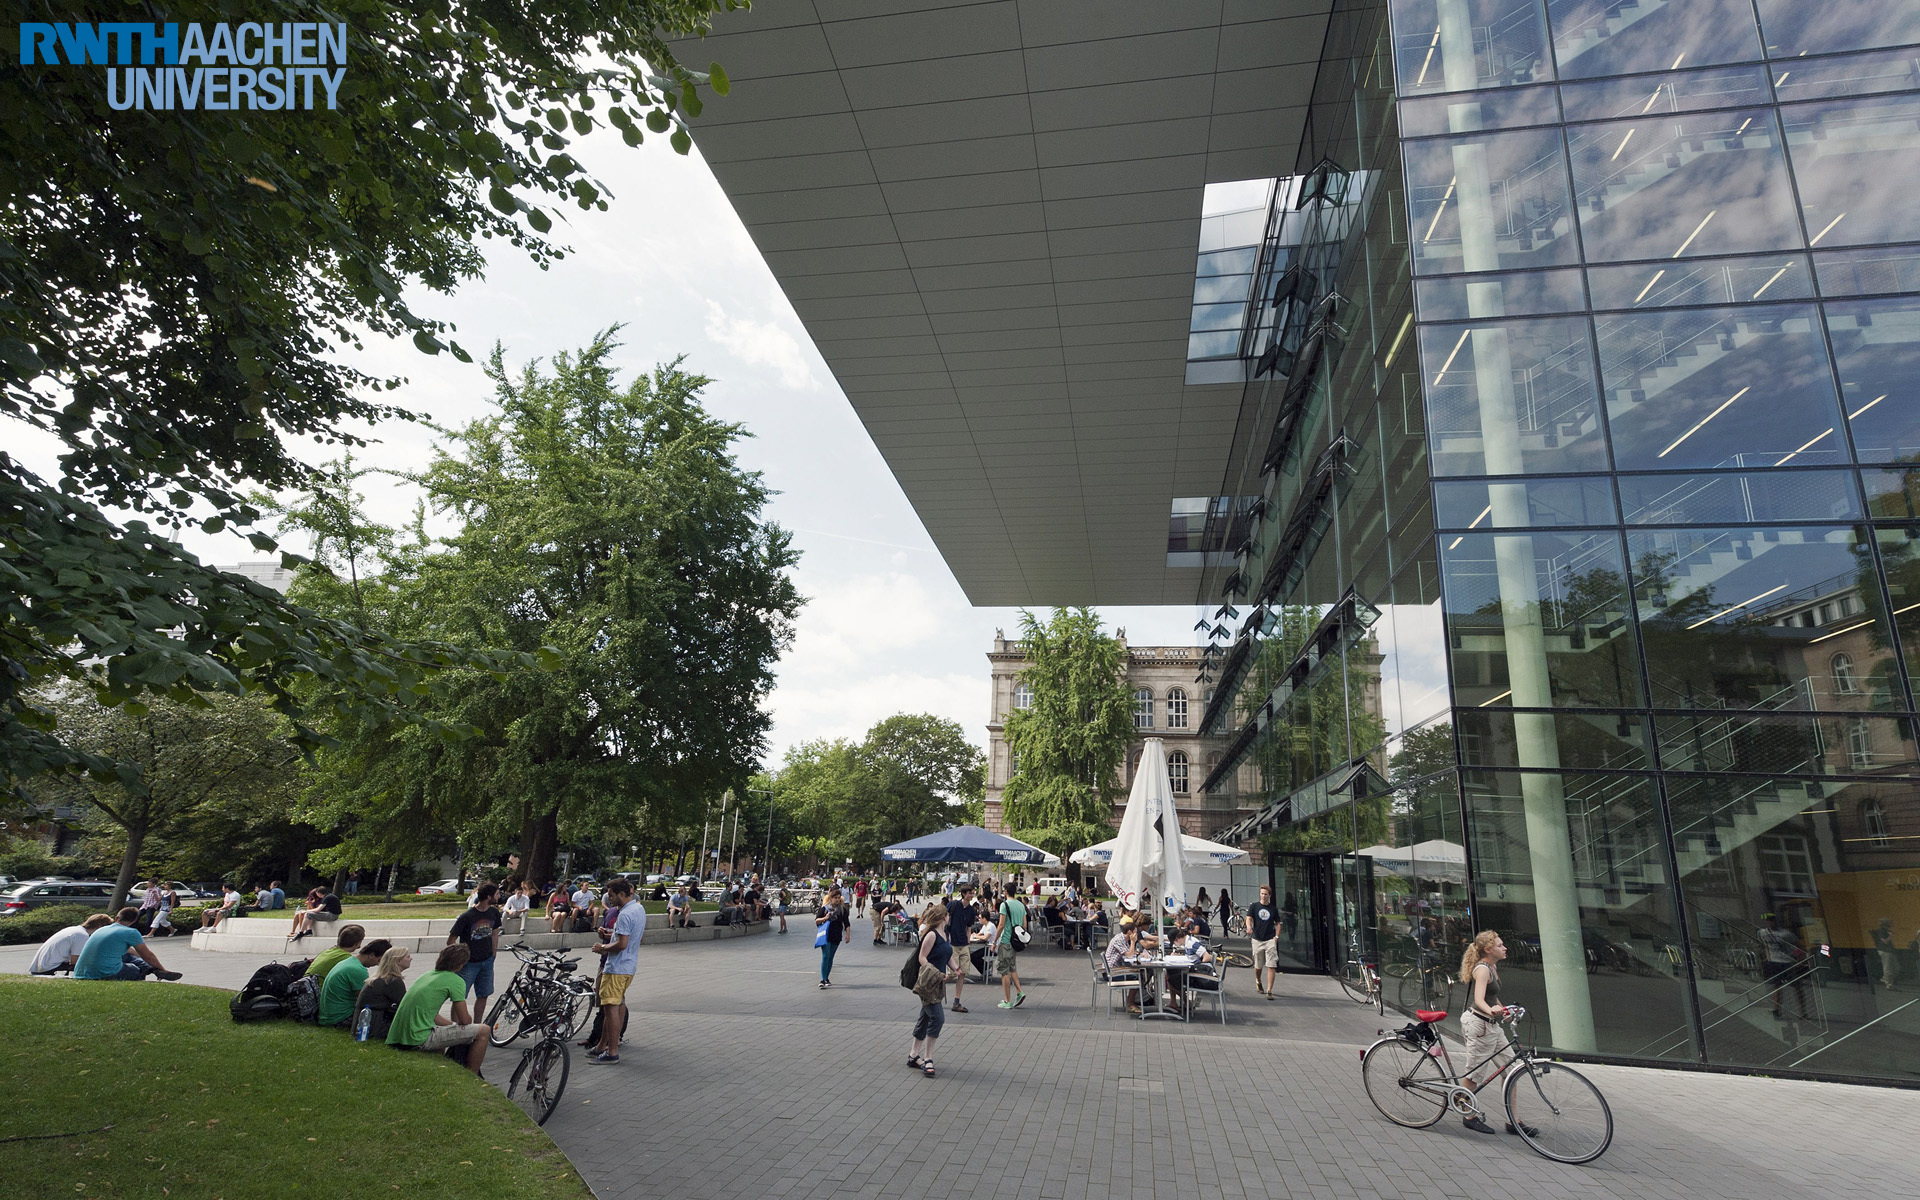
\includegraphics[width = 0.5\textwidth]{Contents/Resources/superc.jpeg}
	\caption[Eine Abbildung (kurze Abbildungsunterschrift ohne Quelle)]{Eine Abbildung (lange Abbildungsunterschrift mit Quelle, Quelle: \cite[1]{Mustermann.2012})}
	\label{fig:eine_abbildung}
\end{figure}

\begin{figure}[htbp]
	\centering
	\begin{subfigure}[t]{0.46\textwidth}
		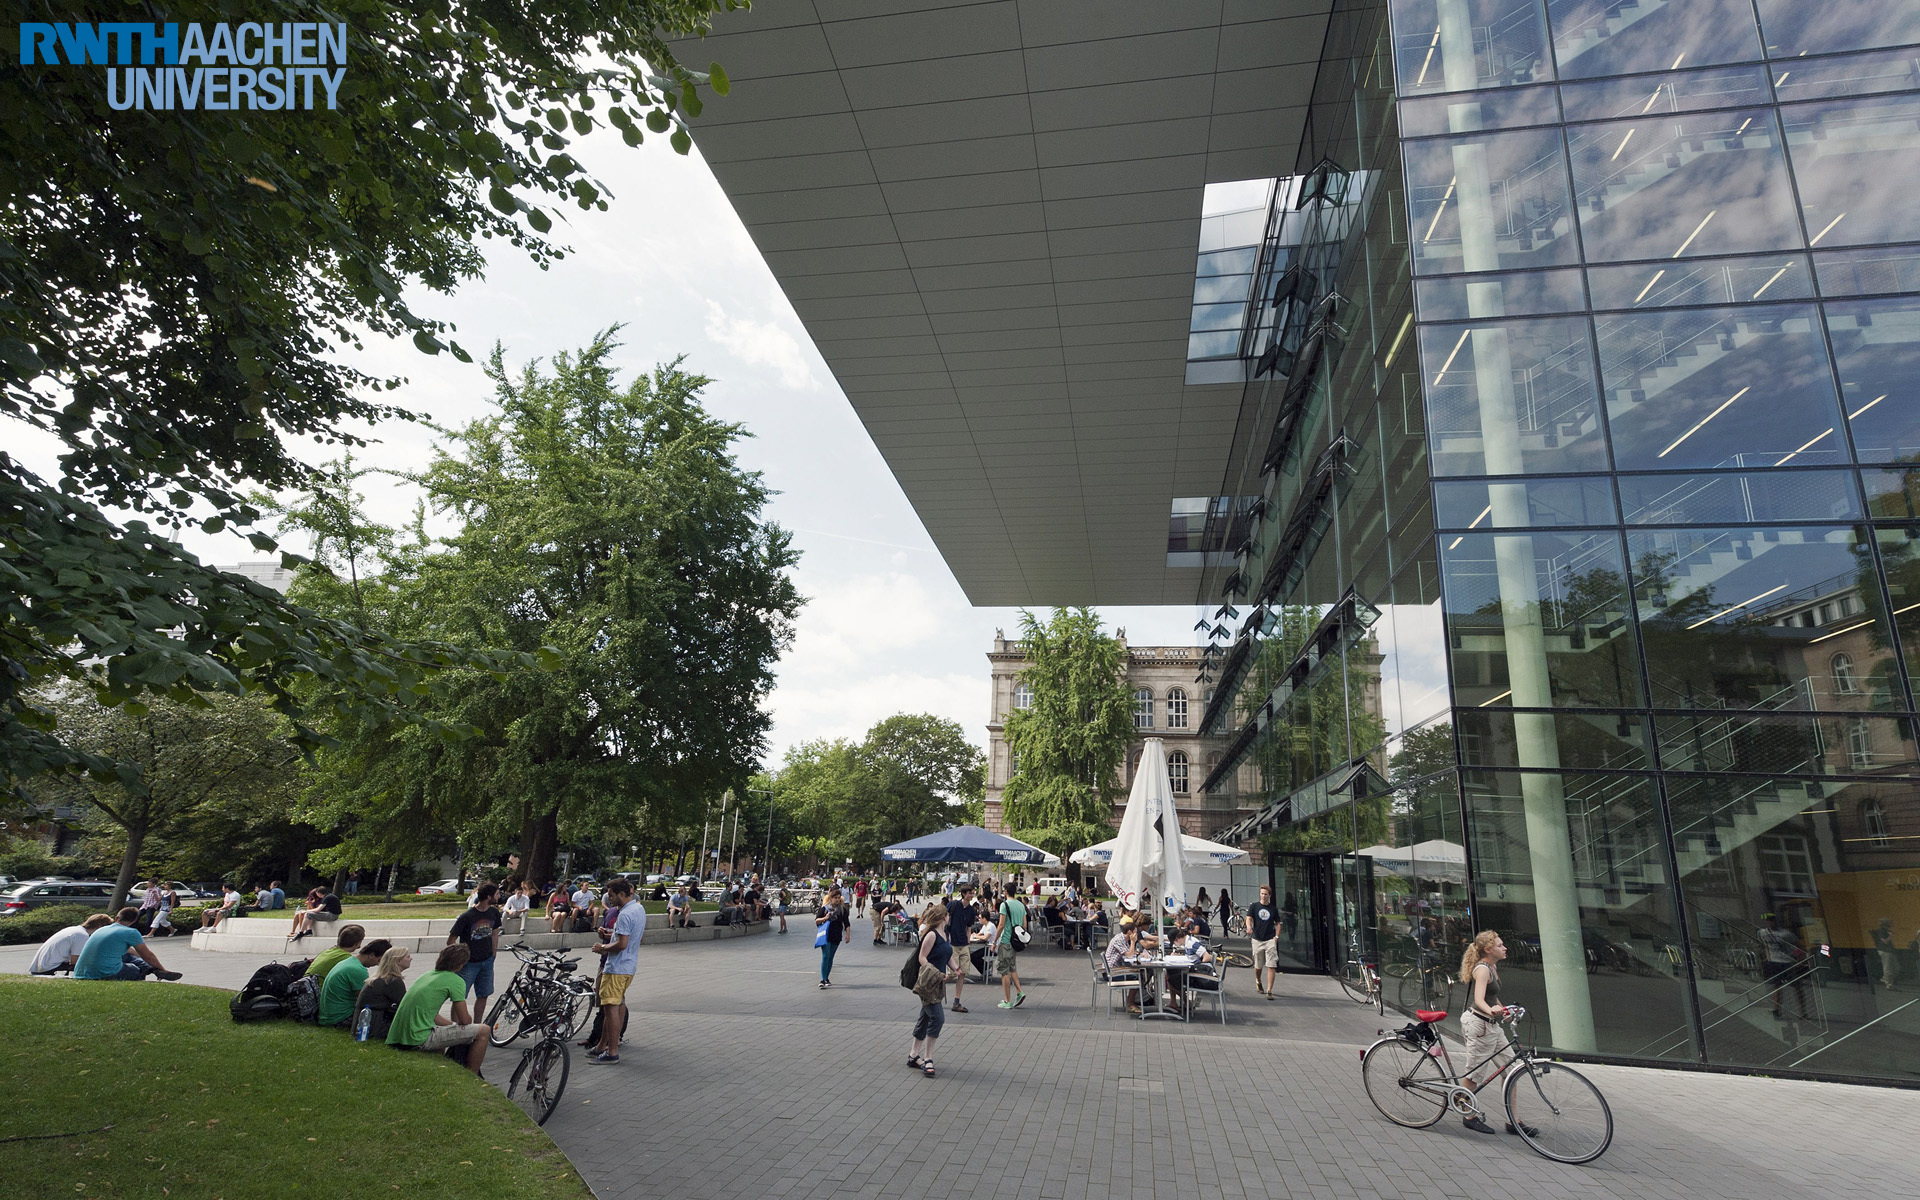
\includegraphics[width = 1\textwidth]{Contents/Resources/superc.jpeg}
		\caption{Bild 1}
		\label{fig:bild1}
	\end{subfigure}
	\begin{subfigure}[t]{0.46\textwidth}
		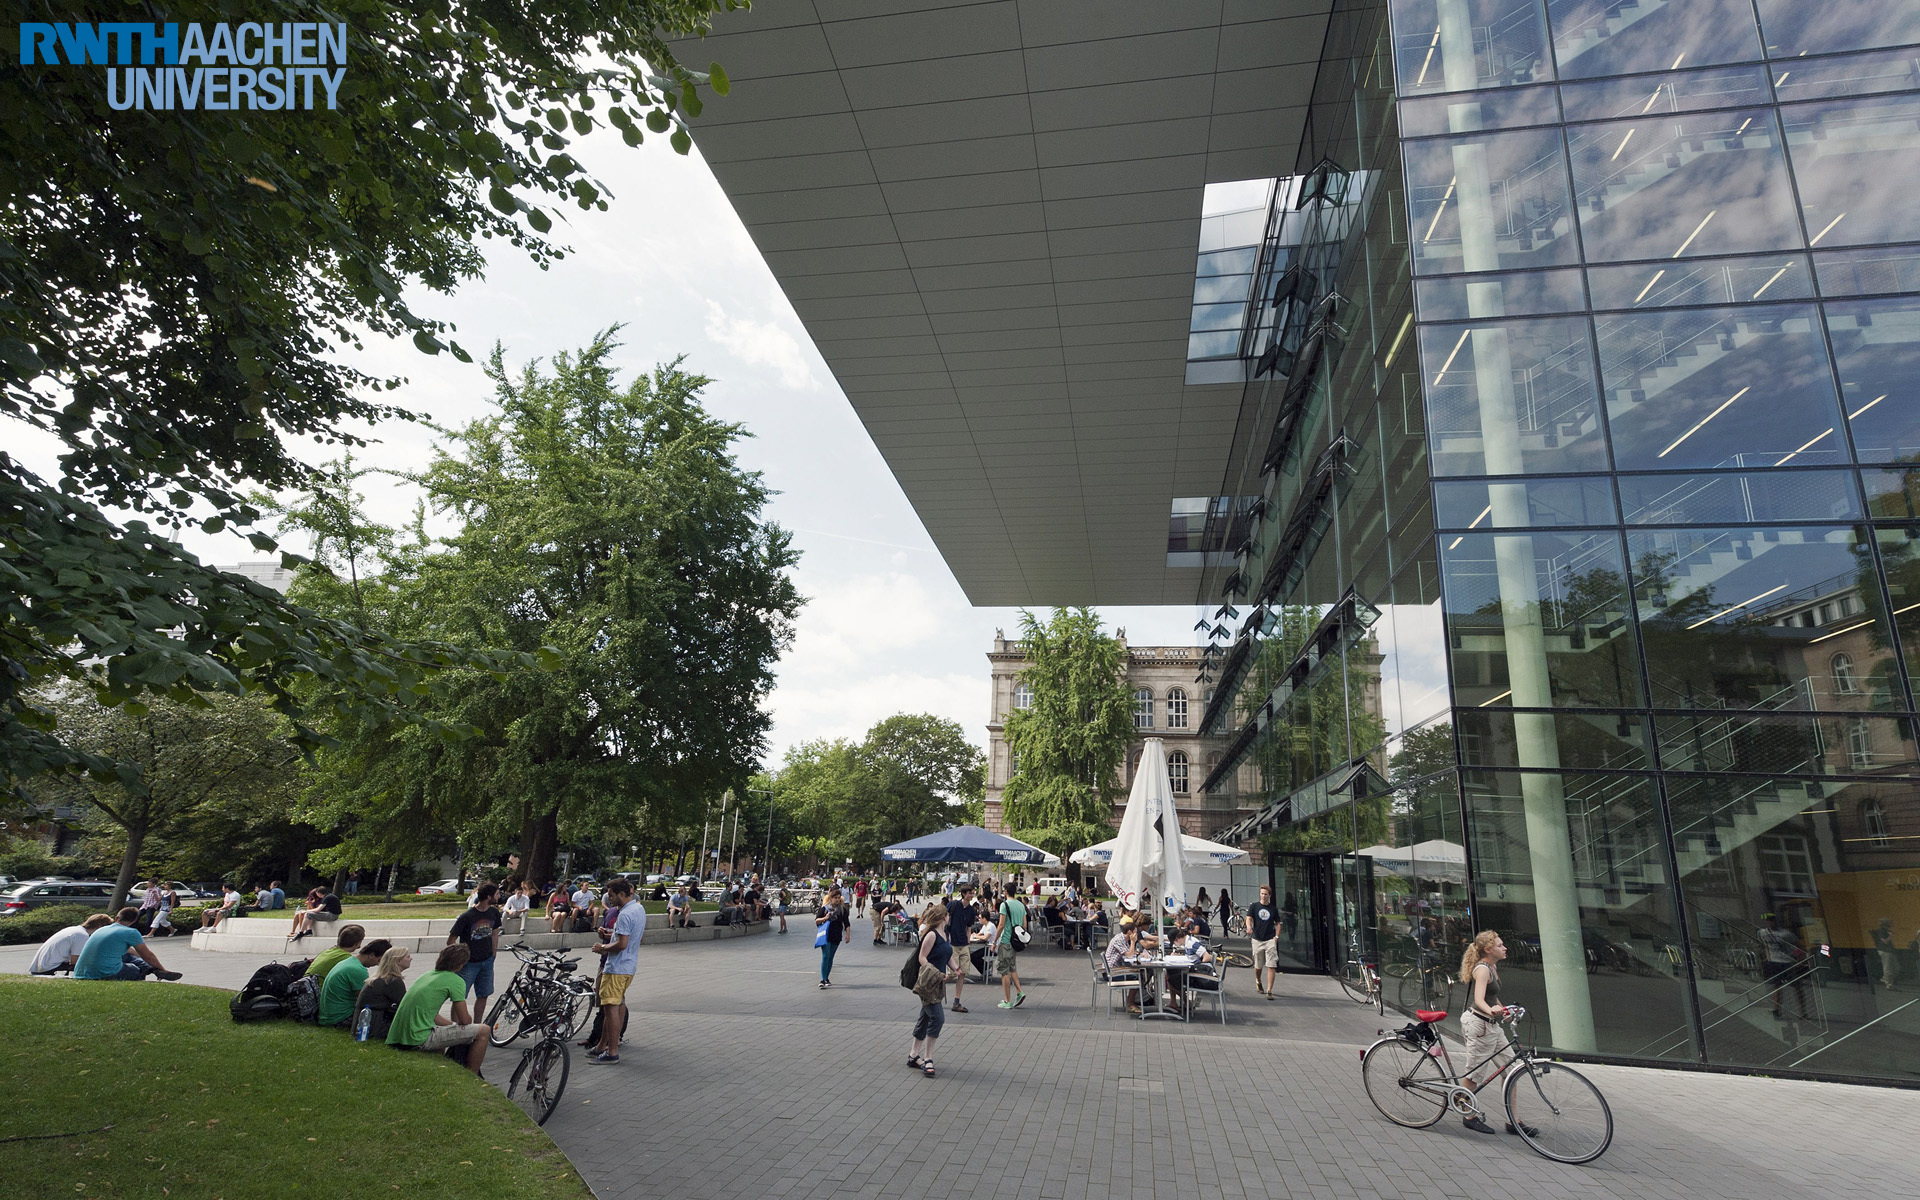
\includegraphics[width = 1\textwidth]{Contents/Resources/superc.jpeg}
		\caption{Bild 2}
		\label{fig:bild2}
	\end{subfigure}
	\caption[Zwei Abbildungen]{Bild 1 (a) und Bild 2 (b)}
	\label{fig:mehrere_abbildungen}
\end{figure}

\cleardoublepage
% Abschnitt 3 --------------------------------------------------------------
% 		Name des Abschnittes
% --------------------------------------------------------------------------
\section{Tabellen}
\label{sec:tabellen}

\begin{table}[htbp]
	\centering	
	\caption{Tabelle mit automatischer Ausrichtung}
		\begin{tabular}{lcr}
	 	\toprule
	 	l & c & r\\
	 	\midrule
		a & b & c\\[0.25em]
		aa & bb & cc\\[0.25em]
		aaa & bbb & ccc\\
		\bottomrule
	\end{tabular}	
	\label{tab:tabelle1}
\end{table}

\begin{table}[htbp]
  \centering
  \caption{Tabelle mit Ausrichtung an Trennungszeichen}
    \begin{tabular}{R{4}{3} R{4}{0}}
    \toprule
          \multicolumn{1}{c}{a} & \multicolumn{1}{c}{b}\\
    \midrule
	1,234 & 1234\\
	12,34 & 123\\
	123,4 & 12\\
	1234  & 1\\
    \bottomrule
    \end{tabular}
  \label{tab:tabelle2}
\end{table}

\begin{table}[htbp]
	\centering	
	\caption{Tabelle mit Zellen über mehrere Zeilen oder Spalten}
		\begin{tabular}{lcr}
	 	\toprule
	 	l & c & r\\
	 	\midrule
		\multicolumn{2}{c}{ab} & c\\[0.25em]
		\multirow{2}{*}{aa} & bb & cc\\[0.25em]
		& bbb & ccc\\
		\bottomrule
	\end{tabular}	
	\label{tab:tabelle3}
\end{table}

%\begin{table}[htbp]
%  \centering
%  \caption{Mehrere Untertabellen}
%  \subtable[Tabelle 1]{
%    \centering  
%\begin{tabular}{lcr}
%	 	\toprule
%	 	l & c & r\\
%	 	\midrule
%		a & b & c\\[0.25em]
%		aa & bb & cc\\[0.25em]
%		aaa & bbb & ccc\\
%		\bottomrule
%	\end{tabular}	
%  }
%  \subtable[Tabelle 2]{
%    \centering  
%\begin{tabular}{lcr}
%	 	\toprule
%	 	l & c & r\\
%	 	\midrule
%		a & b & c\\[0.25em]
%		aa & bb & cc\\[0.25em]
%		aaa & bbb & ccc\\
%		\bottomrule
%	\end{tabular}	
%  }
%\label{tab:tabellen}
%\end{table}

\cleardoublepage
% Abschnitt 4 --------------------------------------------------------------
% 		Name des Abschnittes
% --------------------------------------------------------------------------
\section{Gleichungen}
\label{sec:gleichungen}

\begin{align}
	F = m a 
	\label{eqn:newton}
\end{align}


\section{Anführungszeichen}
\label{sec:anfuehrungszeichen}
Es gibt mehrere Möglichkeiten deutsche Anführungszeichen einzufügen:\\
\glqq test\grqq\\
"`test"'\\

\section{Zitationen}

Zitation einer Quelle: \cite{Mustermann.2012}\\
Zitation einer Quelle mit Seitenangabe: \cite[12-16]{Mustermann.2012}\\
Zitation mehrerer Quellen: \cites{Mustermann.2012}{Musterfrau.2011}\\
Zitation mehrerer Quellen mit Seitenangabe: \cites[12-16]{Mustermann.2012}[3]{Musterfrau.2011}\\

